\documentclass[11pt]{article}
%\usepackage[scaled]{helvet}
\usepackage{amsmath}
\usepackage[utf8]{inputenc}
\usepackage{graphicx}
\usepackage{url}
\usepackage[font={small,it}]{caption}
%\renewcommand\familydefault{\sfdefault}
\renewcommand{\baselinestretch}{1.1}
\usepackage[letterpaper, margin=1in]{geometry}

\title{Udacity Machine Learning Nanodegree\\ CAPSTONE: Photo OCR Prototype}
\author{Wolfgang Steiner \\ \small{wolfgang.steiner@gmail.com}}
\date{January 2017}

\begin{document}
\maketitle
\section{Introduction}
In this capstone project I present the prototype of a photo OCR (optical character recognition)
pipeline based on a sliding window algorithm that is able to automatically detect and parse
text in images. Systems such as this are used in a wide variety of applications
such as the automatic parsing of house numbers from street view photos \cite{Goodfellow2013},
automatic translation of text \cite{} or scanning of documents using a mobile device \cite{}.

The task of photo OCR can be divided into three distinct stages which are shown in Fig.~\ref{fig:pipeline}.
The first stage of this pipeline is text \emph{detection} which aims to determine bounding boxes for each
distinct set of characters in the image. The second stage is character \emph{segmentation}, in which
each bounding box is scanned for character gaps with the aim of finding distinct characters
that can finally be classified in the third stage by the character \emph{classification}.

Each stage of the pipeline consists of a convolutional neural network

In order to reduce the complexity and training time of the project, the pipeline is confined to
only process and parse digits but every stage could be extended and retrained to also handle letters
and other characters.

Similar to the work in \cite{Jaderberg2016} synthetic images have been generated to train the classifiers.


\begin{figure}[ht]
    \centering
    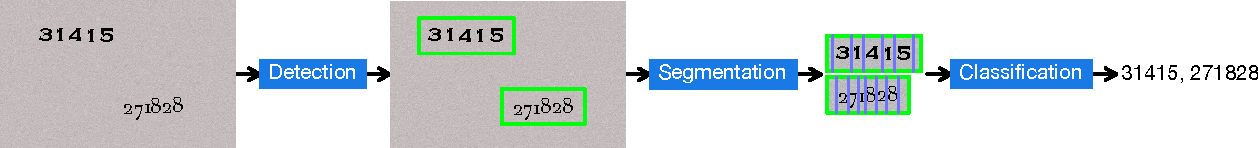
\includegraphics[scale=0.8]{fig/Pipeline}
    \caption{Photo OCR pipeline.}
    \label{fig:pipeline}
\end{figure}

\section{Metrics and Benchmark}
In order to assess the performance of the complete OCR pipeline, a set of test images $x_i$ containing
a randomly generated string of digits of varying length is processed and the extracted string $a(x_i)$ is
compared to the real label $y(x_i)$ using the following metric:
\begin{equation}
  \operatorname{accuracy}(\begin{bmatrix}x_{1}\\x_{2}\\\vdots\\x_{n}\end{bmatrix},\begin{bmatrix}y(x_{1})\\y(x_{2})\\\vdots\\y(x_{n})\end{bmatrix}) = 1 - \frac{\sum\limits_{i=0}^n{\operatorname{min}\left(\operatorname{lev}(y(x_i), a(x_i)), |y(x_i)|\right)}}{\sum\limits_{i=0}^n{|y(x_i)|}}
\end{equation}
Here, $a(x_i)$ is the label (string of digits) predicted by the system and $|y(x_i)|$ is the length of
the i-th true label. $\operatorname{lev}(y(x_i), a(x_i))$ denotes the Levenshtein distance \cite{Levensht20:online} between
the true label and the predicted label. The Levenshtein distance counts the number of edit operations
that are required to make two strings exactly equal by either deleting, inserting or
changing single characters. When calculating the accuracy, the Levenshtein distance is limited to
the length of the true label (by use of the $\operatorname{min}$ function). This prevents the accuracy
of a single example to become negative.

Human level performance on the task of text transcription is often estimated to be greater
than 98\% \cite{Goodfellow2013}. So an obvious benchmark for a OCR system would be to
attain comparable or even better performance than human performance. When extracting text the
performance of the system can be augmented by use of a dictionary to correct badly classified
characters. When dealing with number strings only, this augmentation is not possible and
the accuracy of the OCR system

A second performance benchmark is speed. One application for an OCR system would be text extraction
of documents scanned by use of the camera of a smartphone. The images would then be send to
a server for processing or even better would be precessed directly on the mobile device.
In both cases scanning a photo for text should not take more than a few second. For use in
an augmented reality app, the speed needs to be even faster in order to allow for an acceptable
frame rate. In this case, processing on the mobile device should be faster than about
250ms.


\section{Training Data}
In this project I predominantly used synthetic images. In order to have a large variety of fonts,
I used the google fonts repository as a source \cite{googlefo53:online}. After excluding some
symbol and non-latin fonts, a collection of 1525 fonts was available for synthesizing images.
The procedure for synthesizing training images is as follows:
\begin{itemize}
  \itemsep0em
  \item A text and a background color is chosen randomly.
  \item A background image is synthesized by upscaling noise by a random factor and applying gaussian blurring.
  \item One of the 1525 fonts is chosen randomly.
  \item One of the characters is chosen randomly.
  \item Adjacent characters are added in some images to the left or right.
  \item An outline is randomly added to the characters.
  \item A shadow of random width and direction is added to the characters.
  \item The image is rotated by a random amount.
  \item Gaussian blur is applied with random radius.
  \item Noise of random amount is added to the image.
\end{itemize}

\begin{figure}[ht!]
  \centering
  \makebox[\textwidth][c]
  {
    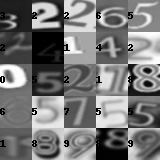
\includegraphics[width=0.35\linewidth]{fig/char_generator_examples}
    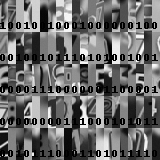
\includegraphics[width=0.35\linewidth]{fig/char_segmentation_examples}
    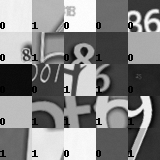
\includegraphics[width=0.35\linewidth]{fig/char_detection_examples}
  }
  \caption
  {
    Examples of synthesized images used to train the character classifier (left), character segmentation
    classifier (center) and character detection classifier (right).
  }
  \label{fig:training_images}
\end{figure}


Some examples of images used to train the three required CNN classifiers are shown in Fig.~\ref{fig:training_images}.
%
In all cases, training and prediction is done with grayscale images with a fixed height of 32~px.
%
Training images are not pre-generated before training but are generated online during training.
%
For this I implemented python generators for the three types of training images that synthesize
batches of images in separate worker threads.
%


Training images for the character classifier (Fig.~\ref{fig:training_images}, left) have characters centered in the images (32x32~px) as will be encountered
by the classifier after segmentation.
%
Characters are also resized to the width of the image as the windows between character boundaries are rescaled to the
input width of 32~px.
%
The labels are simply the corresponding character and are one-hot encoded for training and prediction.


Training images for the segmentation classifier (Fig.~\ref{fig:training_images}, center) are only 8~px wide in order to improve the spacial resolution of the segmentation procedure (see below).
%
Here, label "1" is assigned if a character starts to the right of the center (for the beginning of a character sequence),
a character starts to the left of the center (for the end of a character sequence), or if the spacing
between characters is in the center of the image (for segmenting between characters of a sequence).
%
Label "0" is assigned, if no character is present in the image or if a character is in the center of the image.


Finally, the training images for the character detection classifier (Fig.~\ref{fig:training_images}, right) are
designed to find bounding boxes for character sequences that fit as tight as possible in order to improve
the accuracy of character segmentation and classification.
%
Because of this, images that only have small
text areas and images without characters are labeled "0".
%
Only images that have a high percentage of their area filled by character geometry are labeled "1".

\section{Algorithms and Techniques}
\subsection{Text Detection}
\subsubsection{Sliding Window Algorithm}
The first step in the OCR pipeline is text detection.
%
Here a two dimensional sliding window algorithm is used to detect characters in the image and to fit bounding boxes
around each character sequence encountered.
%
In order to detect text of different sizes, the process of sliding windows is repeated at different
scales.
%
The choice of minimum and maximum scale factors are application specific and directly determine the
biggest/smallest size of text that can be recognized and processed by the following stages of the
pipeline.
%
When scaling the image for one iteration of the sliding window procedure, it is also rescaled
so that its width and height are multiples of 32px, which is the input size of the character detection
classifier.

The image data of each window is then concatenated into an input tensor for the character detection
classifier which has a sigmoid activation function at its output.
%
If the predicted value for a window exceeds a certain threshold (0.95) it is added to a rectangle list that computes
the union of overlapping rectangles.
%
At the end of the procedure, each union of positively classified rectangles is likely to be a bounding
box containing a character sequence which is then segmented into single characters for classification.

\subsubsection{Character Detection Classifier}






\subsection{Character Segmentation}
\subsubsection{Sliding Window Algorithm}
\begin{figure}[ht]
    \centering
    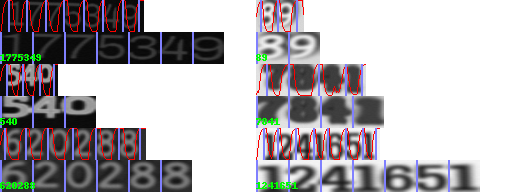
\includegraphics[width=1.1\linewidth]{fig/segmentation}
    \caption{
      Examples of the character segmentation. The top row of each example shows the input
      image. The score of the segmentation classifier is visualized in red, with each dot representing
      the output for one sliding window iteration. The resulting character border is shown in green.
      The bottom row shows the character images that have been extracted and rescaled based on the
      segmentation. These images are then fed into the character classifier. }
    \label{fig:segmentation}
\end{figure}
\subsubsection{Character Segmentation Classifier}


\subsection{Character Classification}

\section{Methodology}


\section{Results}
\begin{figure}[ht]
    \centering
    \makebox[\textwidth][c]
    {
        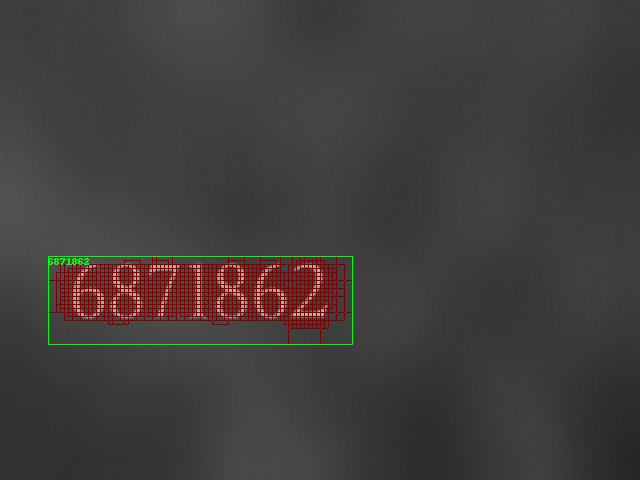
\includegraphics[width=0.35\linewidth]{fig/good_examples_pipeline/4f030f3c-5576-48bf-a83f-8d11534dfdd5}
        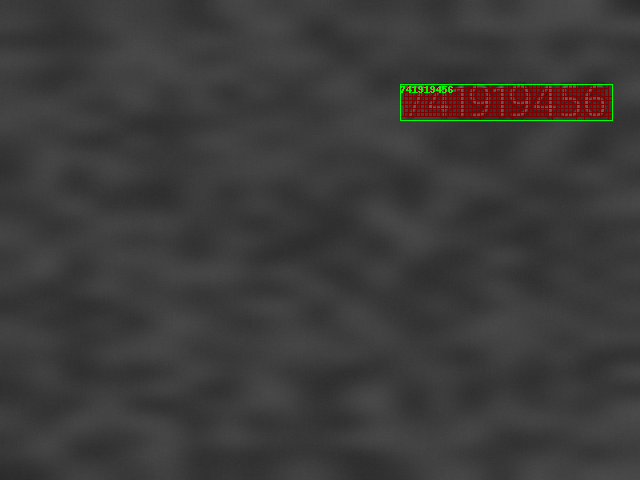
\includegraphics[width=0.35\linewidth]{fig/good_examples_pipeline/c53b3f16-079b-46bf-90cb-6a7a2cfef5f5}
        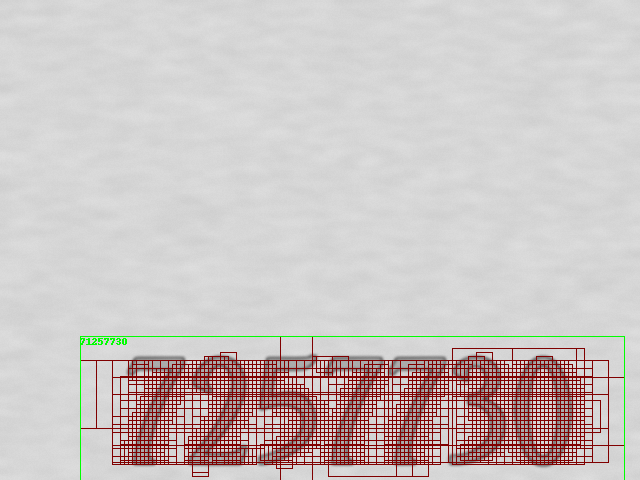
\includegraphics[width=0.35\linewidth]{fig/good_examples_pipeline/95e76bd2-5815-4d36-aea1-7a5712ec0ae9}
    }
    \caption{Examples of correctly extracted digits strings. Red rectangles are positive classifications of the
    character detection classifier. The green rectangle corresponds to the bounding box calculated as the union
    of the red rectangles.}
    \label{fig:good_examples_pipeline}
\end{figure}

\begin{figure}[ht]
    \centering
    \makebox[\textwidth][c]
    {
      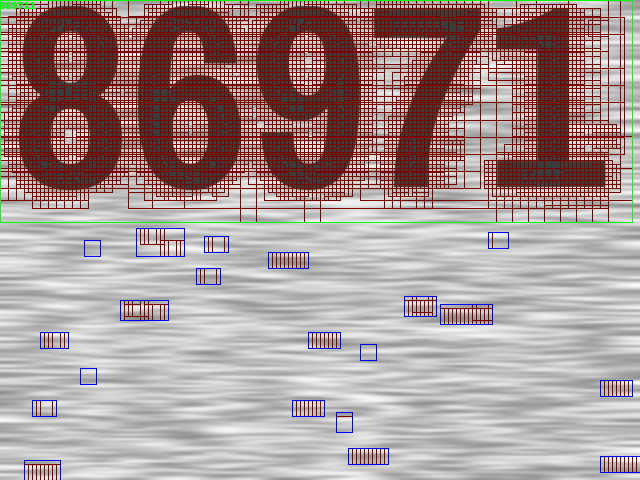
\includegraphics[width=0.35\linewidth]{fig/bad_examples_pipeline/cf163c7f-3326-49e9-a700-cd560bdff920}
      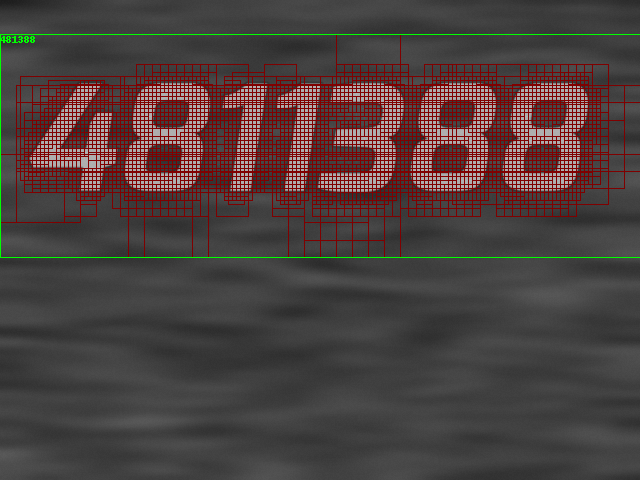
\includegraphics[width=0.35\linewidth]{fig/bad_examples_pipeline/aac7a8dd-a27e-4888-a467-803332236945}
      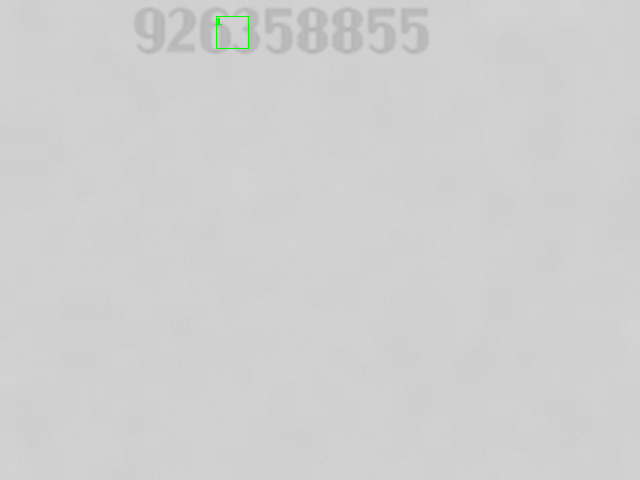
\includegraphics[width=0.35\linewidth]{fig/bad_examples_pipeline/c884bc67-4128-43e7-8ff5-814f79e79699}
    }
    \caption{
      Examples of incorrectly extracted digits strings. Repetition of digits (left).
      Missing digits (center). Low contrast images and small test size may result in character failing detection,
      resulting in a bounding box that is too small for segmentation and classification (right).
    }
    \label{fig:bad_examples_pipeline}
\end{figure}




\newpage
\bibliography{main,web}
\bibliographystyle{ieeetr}

\end{document}
